\documentclass{article}
\usepackage[utf8]{inputenc}
\usepackage[margin=1in]{geometry}

\usepackage{algorithm}
\usepackage[noend]{algpseudocode}
\usepackage{enumitem}

\usepackage{tikz}
\usetikzlibrary{calc,shapes.multipart,chains,arrows,positioning}
\tikzstyle{vertex}=[draw,fill=myseagreen,circle,minimum size=24pt,inner sep=0pt]
\definecolor{myseagreen}{RGB}{240,240,240}

\title{Strongly Connected Components}
\author{Kevin Geng and Lawrence Wang}
\date{27 January 2017}

\begin{document}

\maketitle

\section{Introduction}

Let's start by considering connectivity in undirected graphs. In such a graph, two nodes $u$ and $v$ are connected if there is some path from $u$ to $v$. Correspondingly, a connected component in such a graph is a subgraph in which every node is reachable from every other node. Finding such components is straightforward: we can simply perform a DFS. If we want to be able to connect components dynamically, we can use the Union-Find data structure.

\begin{figure}[h]
\center
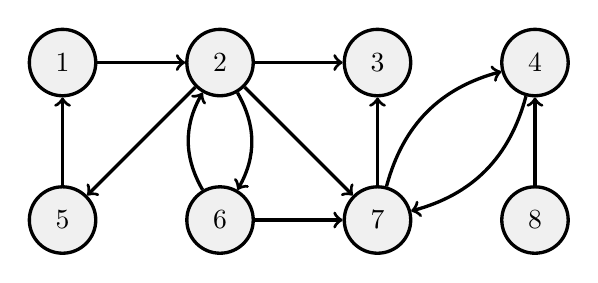
\begin{tikzpicture}[very thick,level/.style={sibling distance=70mm/#1}]
\draw (0, 0) node [vertex] (n1) {5};
\draw (2, 0) node [vertex] (n2) {6};
\draw (4, 0) node [vertex] (n3) {7};
\draw (6, 0) node [vertex] (n4) {8};
\draw (0, 2) node [vertex] (m1) {1};
\draw (2, 2) node [vertex] (m2) {2};
\draw (4, 2) node [vertex] (m3) {3};
\draw (6, 2) node [vertex] (m4) {4};
\draw[->] (m1) -- (m2);
\draw[->] (m2) -- (n1);
\draw[->] (n1) -- (m1);
\draw[->] (n2) edge [bend left] (m2);
\draw[->] (m2) edge [bend left] (n2);
\draw[->] (n2) -- (n3);
\draw[->] (m2) -- (m3);
\draw[->] (m2) -- (n3);
\draw[->] (n3) -- (m3);
\draw[->] (n3) edge [bend left] (m4);
\draw[->] (m4) edge [bend left] (n3);
\draw[->] (n4) -- (m4);
\end{tikzpicture}
\caption{A directed graph. \textit{Credit: Crash Course Coding Companion.}}
\end{figure}

If our graph is directed, however, our previous definition of connectivity poses a problem. If $v$ is reachable from $u$, this doesn't imply that $u$ is reachable from $v$. So instead, we'll say that $u$ and $v$ are \textit{strongly connected} if they are both reachable from each other.\footnote{Two nodes in a directed graph are \textit{weakly connected} if at least one is reachable from the other --- as if you just replaced every directed edge with an undirected edge.} Extending this to the idea of connected components, a \textit{strongly connected component} is a subgraph where any two nodes in this subgraph are strongly connected.


\section{Kernel graph}

We can travel between any two nodes in the same strongly connected component. So what if we replaced each strongly connected component with a single node? This would give us what we call the \textit{kernel graph}, which describes the edges between strongly connected components. Note that the kernel graph is a directed acyclic graph (why?). This means that there are orderings of the nodes, where if node $A$ comes before node $B$ in our ordering, then it is impossible to get to $A$ from $B$ by traversing along edges. 

\begin{figure}[h]
\center
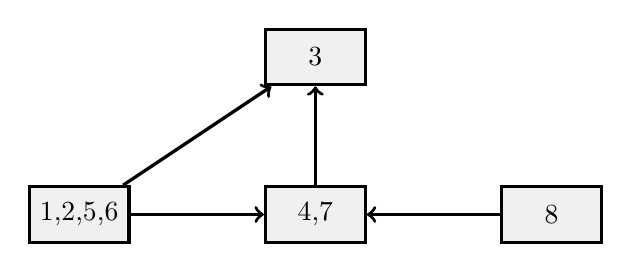
\begin{tikzpicture}[very thick,level/.style={sibling distance=70mm/#1}]
\tikzstyle{vertex}=[draw,fill=myseagreen,rectangle,minimum width=36pt,minimum height=20pt,inner sep=0pt]
\draw (0, 0) node [vertex] (n1) {1,2,5,6};
\draw (3, 0) node [vertex] (n3) {4,7};
\draw (6, 0) node [vertex] (n4) {8};
\draw (3, 2) node [vertex] (n2) {3};
\draw[->] (n1) -- (n3);
\draw[->] (n1) -- (n2);
\draw[->] (n3) -- (n2);
\draw[->] (n4) -- (n3);
\end{tikzpicture}
\caption{Kernal graph of the above directed graph.}
\end{figure}


\section{Kosaraju-Sharir algorithm}

First, let's reverse all of the edges of the original graph to get the reverse graph. Perform a postorder traversal on this graph using DFS, and store the reverse of the postorder in a list. This is similar to a topological sort of the reverse graph.

Then, we simply perform an ordinary flood-fill DFS on the graph, but looping through the nodes in the order given above. All we need to do is assign components in the order in which we visit them, and this gives us the strongly connected components! To understand why, consider what we've done in terms of the kernel graph. Each component that we flood-fill is unreachable from any other unvisited component.


\begin{algorithm}[H]
\caption{Kosaraju-Sharir}
\begin{algorithmic}
\Function{Visit}{vertex $u$}
    \If {$u$ has not been visited}
		\State mark $u$ as visited
	    \ForAll{in-neighbors $v$ of $u$} \Comment such that $v \rightarrow u$
			\State \Call{Visit}{$v$}
		\EndFor
		\State add $v$ to front of $L$
	\EndIf
\EndFunction
\Function{Assign}{vertex $u$, $num$}  \Comment flood-fill an entire component
    \State $id(u) \gets num$
    \ForAll{out-neighbors $v$ of $u$} \Comment such that $u \rightarrow v$
        \State \Call{Assign}{$v$, $num$}
    \EndFor
\EndFunction
\Function{KosarajuSharir}{$G(V,E)$}
	\State initialize new empty list $L$
	\ForAll{vertices $v \in V$}
		\State \Call{Visit}{$v$}
	\EndFor
	\State $num \gets 0$
	\ForAll{vertices $v \in L$}
	    \If{$id(v)$ is undefined} \Comment $v$ has not been visited
	        \State $num \gets num + 1$
	        \State \Call{Assign}{$v$, $num$}
	    \EndIf
	\EndFor
\EndFunction
\end{algorithmic}
\end{algorithm}

\section{Tarjan's Algorithm}

Kosaraju-Sharir requires two traversals through the entire graph. We can find strongly connected components with only one traversal using Tarjan's algorithm, though it is more difficult to implement. Essentially, the algorithm performs a DFS traversal while adding visited nodes to a stack. A node remains on the stack \textit{iff} it can reach a higher node on the stack; otherwise, it is the root node in the search tree of its component.


\section{Problems}

\begin{itemize}[leftmargin=0pt]
\item[\label={}]
\textit{Mowing the Field} (USACO January 2016, Platinum)

In an effort to better manage the grazing patterns of his cows, Farmer
John has installed one-way cow paths all over his farm.  The farm
consists of $N$ fields ($1 \le N \le 100000$), conveniently numbered $1..N$, with each one-way
cow path connecting a pair of fields. For example, if a path connects
from field $X$ to field $Y$, then cows are allowed to travel from $X$ to $Y$
but not from $Y$ to $X$.

Bessie wonders how much grass she will be able to eat if she
breaks the rules and follows up to one path in the wrong direction.
Please compute the maximum number of distinct fields she can visit
along a route starting and ending at field $1$, where she can follow up
to one path along the route in the wrong direction.  Bessie can only
travel backwards at most once in her journey.  In particular, she
cannot even take the same path backwards twice.

\end{itemize}

\end{document}
